% circuit_overlay.tex — GENERATED by scripts/gen_overlay_tex.py, do not hand-edit.
% Build:  pdflatex circuit_overlay.tex
\documentclass[11pt]{article}
\usepackage[a4paper,margin=18mm]{geometry}
\usepackage{tikz}
\usepackage{xcolor}
\usepackage{booktabs}
\usepackage{helvet}
\renewcommand{\familydefault}{\sfdefault}
\usepackage[T1]{fontenc}
\usetikzlibrary{calc}
\setlength{\parindent}{0pt}

\definecolor{gov}{HTML}{0D6B73}      % governed by a streamed parameter
\definecolor{ungov}{HTML}{78848F}    % in the circuit, never estimated
\definecolor{sensor}{HTML}{B1541F}
\definecolor{ink}{HTML}{131820}
\definecolor{ink2}{HTML}{4C5866}

% pins: a small dot at the anatomical point, the number in a chip.
% \pinX{n}{x}{y} puts the number on the point; \leadX{n}{px}{py}{lx}{ly} draws a leader.
\newcommand{\pinG}[3]{\filldraw[gov,draw=white,line width=.5pt] (#2,#3) circle (1.9mm)
  node[white,font=\bfseries\sffamily\fontsize{5}{5}\selectfont] {#1};}
\newcommand{\pinU}[3]{\filldraw[white,draw=ungov,line width=.6pt] (#2,#3) circle (1.8mm)
  node[ungov,font=\bfseries\sffamily\fontsize{5}{5}\selectfont] {#1};}
\newcommand{\pinS}[3]{\filldraw[sensor,draw=white,line width=.5pt] (#2,#3) circle (1.9mm)
  node[white,font=\bfseries\sffamily\fontsize{5}{5}\selectfont] {#1};}
\newcommand{\leadG}[5]{\draw[gov,line width=.4pt] (#2,#3) -- (#4,#5);
  \filldraw[gov] (#2,#3) circle (0.5mm); \pinG{#1}{#4}{#5}}
\newcommand{\leadU}[5]{\draw[ungov,line width=.4pt] (#2,#3) -- (#4,#5);
  \filldraw[ungov] (#2,#3) circle (0.5mm); \pinU{#1}{#4}{#5}}
\newcommand{\leadS}[5]{\draw[sensor,line width=.4pt] (#2,#3) -- (#4,#5);
  \filldraw[sensor] (#2,#3) circle (0.5mm); \pinS{#1}{#4}{#5}}

\begin{document}

{\sffamily\bfseries\Large Cerebral circuit anatomy\par}
\vspace{1mm}
{\color{ink2}\small The 21 components of the Model~6 outflow segmentation, pinned to the body.
Filled pins are governed by a streamed parameter (8 of 21); hollow pins are in the circuit and
\textbf{never estimated} --- hollow means unmeasured, not normal.\par}
\vspace{4mm}

\begin{center}
\begin{tikzpicture}
  \node[anchor=south west,inner sep=0] (img)
    {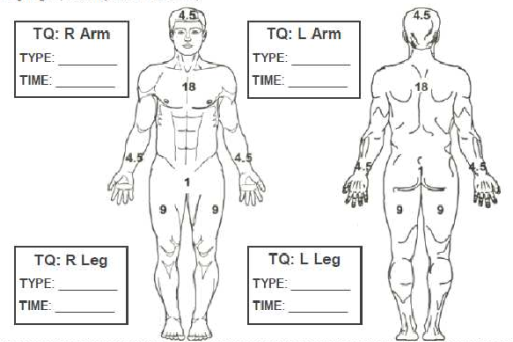
\includegraphics[width=0.94\textwidth]{body_template.png}};
  \begin{scope}[x={(img.south east)},y={(img.north west)}]
    % --- mask the casualty-card tourniquet fields
    \fill[white] (0.0078,0.7193) rectangle (0.24951,0.95906);
    \fill[white] (0.46004,0.7193) rectangle (0.69396,0.95906);
    \fill[white] (0.0078,0.09357) rectangle (0.24951,0.33333);
    \fill[white] (0.46004,0.09357) rectangle (0.69396,0.33333);
    % --- dim the template so the overlay reads as the content
    \fill[white,opacity=0.45] (0,0) rectangle (1,1);
    % --- component pins
    \leadG{1}{0.34698}{0.91228}{0.2729}{0.95322}
    \leadG{2}{0.36842}{0.89474}{0.2729}{0.90351}
    \leadU{3}{0.38986}{0.88889}{0.44444}{0.91228}
    \leadU{4}{0.34308}{0.87427}{0.2729}{0.8538}
    \leadU{5}{0.36257}{0.86257}{0.44444}{0.8655}
    \leadU{6}{0.39181}{0.91813}{0.44444}{0.95906}
    \leadU{7}{0.36842}{0.84211}{0.2729}{0.80409}
    \leadU{8}{0.35088}{0.83333}{0.2729}{0.75439}
    \leadU{9}{0.34503}{0.82164}{0.2729}{0.70468}
    \leadG{10}{0.33918}{0.80409}{0.2729}{0.65497}
    \pinU{11}{0.37817}{0.72222}
    \pinG{12}{0.82456}{0.95906}
    \pinG{13}{0.80117}{0.9386}
    \pinG{14}{0.84016}{0.83918}
    \pinU{15}{0.84211}{0.69591}
    \pinG{16}{0.82456}{0.66959}
    \pinU{17}{0.79727}{0.71637}
    \pinU{18}{0.80117}{0.62573}
    \pinG{19}{0.82456}{0.5614}
    \pinU{20}{0.846}{0.60819}
    \pinU{21}{0.85965}{0.53216}
    % --- sensor sites (SENSORS.md tier 1); comment out this block to hide
    \leadS{S1}{0.36842}{0.93567}{0.44444}{0.81871}
    \leadS{S2}{0.39571}{0.8655}{0.44444}{0.77193}
    \leadS{S3}{0.39766}{0.80409}{0.44444}{0.72515}
    \pinS{S4}{0.25731}{0.48538}
  \end{scope}
\end{tikzpicture}
\end{center}

\vspace{-2mm}
{\small\color{ink2}%
\tikz[baseline=-.5ex]\filldraw[gov] (0,0) circle (1.6mm); governed by a streamed parameter \quad
\tikz[baseline=-.5ex]\filldraw[white,draw=ungov,line width=.7pt] (0,0) circle (1.5mm); in the circuit, never estimated \quad
\tikz[baseline=-.5ex]\filldraw[sensor] (0,0) circle (1.6mm); sensor placement site\par}

\vspace{3mm}
{\footnotesize\color{ink2}\textbf{The pins are schematic.} They mark the anatomical region each
lumped element stands for, not a surgical landmark: \texttt{vertebral\_plexus} is one node for a
network spanning the whole spinal canal, and \texttt{systemic\_venous} is a boundary condition
rather than a place. The tourniquet fields of the source template are masked --- this is an
engineering diagram, not a casualty card, and it carries no triage or treatment meaning.\par}

\vspace{5mm}
{\sffamily\bfseries\large Key\par}
\vspace{2mm}
\begin{tabular}{@{}r l l l r@{}}
\toprule
\# & Component & State / element & Governed by & Share \\
\midrule
1 & Cerebral arterial bed & \texttt{\small V\_a / C\_a} & {\small arterial\_compliance} & 1 \\
2 & Intracranial CSF / brain & \texttt{\small Pic (the measured ICP)} & {\small craniospinal\_compliance} & 0.3 \\
3 & Cerebral venous compartment & \texttt{\small Pv / V\_v} & {\small \color{ungov}not estimated} & --- \\
4 & Arteriolar bed & \texttt{\small Ra} & {\small \color{ungov}not estimated} & --- \\
5 & Capillary bed & \texttt{\small Rc} & {\small \color{ungov}not estimated} & --- \\
6 & Cerebral venous outflow & \texttt{\small Rv} & {\small \color{ungov}not estimated} & --- \\
7 & Craniospinal CSF channel & \texttt{\small Rspine} & {\small \color{ungov}not estimated} & --- \\
8 & Sinus to jugular bulb & \texttt{\small Rss} & {\small \color{ungov}not estimated} & --- \\
9 & Jugular bulb & \texttt{\small P\_j} & {\small \color{ungov}not estimated} & --- \\
10 & Internal jugular vein & \texttt{\small Rijvs (tube law)} & {\small jugular\_resting\_area} & 1 \\
11 & Systemic venous return & \texttt{\small P\_sys} & {\small \color{ungov}not estimated} & --- \\
12 & Dural venous sinus & \texttt{\small Psinus} & {\small sagittal\_sinus\_pressure} & 1 \\
13 & CSF absorption, cranial & \texttt{\small Ro = 0.069*Ro\_tot} & {\small csf\_outflow\_resistance} & 0.069 \\
14 & Vertebral venous collateral & \texttt{\small Rvvs} & {\small collateral\_outflow\_resistance} & 1 \\
15 & Vertebral venous plexus & \texttt{\small P\_vv} & {\small \color{ungov}not estimated} & --- \\
16 & Spinal dural sac & \texttt{\small Psas} & {\small craniospinal\_compliance} & 0.7 \\
17 & Azygos return & \texttt{\small Razy} & {\small \color{ungov}not estimated} & --- \\
18 & Paravertebral / azygos & \texttt{\small P\_px} & {\small \color{ungov}not estimated} & --- \\
19 & CSF absorption, spinal & \texttt{\small Ro\_spine = 0.931*Ro\_tot} & {\small csf\_outflow\_resistance} & 0.931 \\
20 & Vertebral plexus drainage & \texttt{\small Rivp / Revp} & {\small \color{ungov}not estimated} & --- \\
21 & Plexus to systemic shunt & \texttt{\small Rt} & {\small \color{ungov}not estimated} & --- \\
\bottomrule
\end{tabular}

\vspace{4mm}
{\sffamily\bfseries\large Sensor sites\par}
\vspace{2mm}
\begin{tabular}{@{}r l@{}}
\toprule
\# & Placement \\
\midrule
S1 & ICP monitor (bolt or EVD) \\
S2 & Transducer reference (tragus) \\
S3 & Bilateral jugular compression \\
S4 & Arterial line (radial) \\
\bottomrule
\end{tabular}

\vspace{5mm}
{\footnotesize\color{ink2}Components read from \texttt{scripts/circuit.py} (9 compartments,
12 interfaces, 8 \texttt{GOVERNS} entries). Sensor sites follow \texttt{SENSORS.md} tier~1.
Anatomical placement is not part of the segmentation data.\par}

\end{document}
